\section{Neural Networks in Chess}
\label{sec:NeuralNets}

Over the last decade computer engines went from consisting of intelligent efficient search and evaluation algorithms, to being focused on creating larger, and intricate neural network architectures that could reach newer heights when it comes to accuracy and general strength of play. Examples of this include the previously mentioned Stockfish \cite{stockfish2024} and AlphaZero \textbf{REF TO ALPHA ZERO}. The prior being an amalgamation of using algorithms like MinMax \& Alpha-Beta Pruning \ref{sec:Chess Programming} to guide the neural network in finding the most optimal move, while the latter being made up of a neural network that teaches itself the game of chess without prior outside knowledge, using techniques like Monte Carlo Tree Search \textbf{REF TO MCTS}. Both approaches present the different paradigms of creating a strong chess engine, which in turn raises the question "How can one make use of these neural networks to improve how Endgames are played by engines?"

\subsection{Overview}
The main objective of this paper, as highlighted by its title, is to explore how neural networks can be used as a replacement to endgame tablebases in the hope of finding benefits when it comes to the speed of probing, but more importantly to save on the storage space required by the tablebases. For the sake of simplicity and lack of resources, this paper will look into one metric provided by tablebases, and using a neural network in place of the tablebase for probing.

More concretely, the objective is to design a neural network that given a chess position can predict the correct WDL value. Once this is proven feasible, the other metrics can be predicted by the same process. 

\subsection{Pattern Recognition}
\label{subsec:PattRec}
Similar to the approach of considering how a Grandmaster would think about the problem of finding the best move in section \ref{sec:Chess Programming} in order to come up with efficient algorithms for finding the best move, using this approach here when given a position and determining the WDL, more abstractly determining whether it is good or bad, can help pinpoint what features make up a position.

In the experiments conducted by de Groot \cite{deGroot} players of varying strength ranging from masters to complete novices were presented with various positions that could arise in a standard game of chess and were given the task of reproducing the position on an empty board after viewing it for a short period of time (3-10 seconds). On average, it was found that master level players were able to more accurately reproduce the position with only a couple of pieces being misplaced if at all, while novice players showcased having a larger margin of error when recreating the given positions.

On first glance, one could hypothesise that since a master player has spent a long period of time in contact with chess positions that their memory for remembering such positions would be better compared to that of a novice player. Nevertheless, this would be disproven when considering the second set of experiments conducted.

In the second set of experiments both the master and novice player where once again presented with the same task, but this time instead of the positions being those that could come up in a standard game, the players were presented positions where the pieces were placed completely randomly. This time around, the accuracy of the master players significantly dropped in contrast to the first experiment, and was barely better than that of the novice players.

\begin{figure}[H]
    \centering
    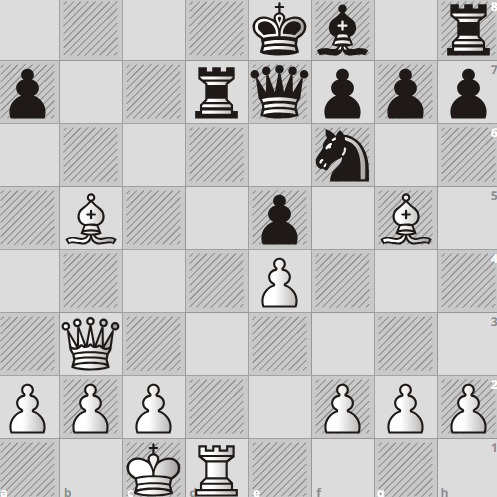
\includegraphics[scale=0.45]{images/MorphyPosition.png}
    \caption{Example of a position that could arise in a game}
    \label{MorphyPosition}
\end{figure}

\begin{figure}[H]
    \centering
    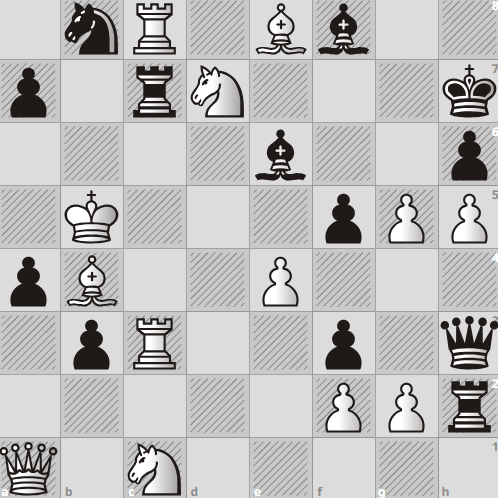
\includegraphics[scale=0.45]{images/RandomPosition.png}
    \caption{Example of a position where the pieces are randomly placed}
    \label{RandomPosition}
\end{figure}

Figures \ref{MorphyPosition} \& \ref{RandomPosition} show visually what a position that could arise from a game, and a random position look like. In fig.\ref{MorphyPosition} a master player would look at symmetrical pawn structure of white, at the e4 pawn being attacked by the Knight, and the pins (meaning a piece can or should not move when being attacked due to it covering a piece of greater value) placed on the d7 Rook and f6 Knight by the b5 and g5 Bishops respectively. While in fig.\ref{RandomPosition} the pieces are not \textit{harmonious} with each other and are scattered haphazardly, making it harder to extract the relations and patterns between them. Figure \ref{MorphyAnotated} demonstrates this.

\begin{figure}[H]
    \centering
    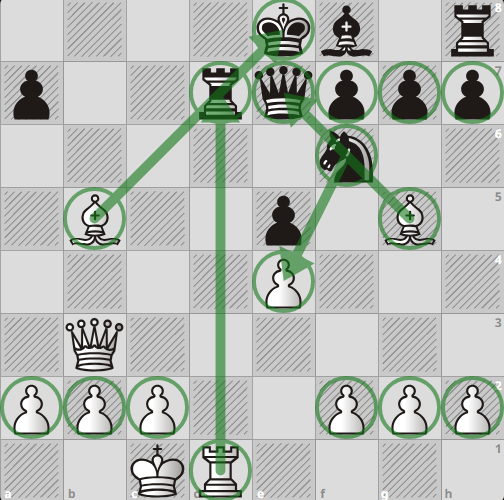
\includegraphics[scale=0.45]{images/MorphyAnotated.png}
    \caption{The patterns a master player would see when observing the position in fig.\ref{MorphyPosition}}
    \label{MorphyAnotated}
\end{figure}

The process just described is exactly what needs to be done by the neural networks, in order to extract the essential features like pawn structures, relative positions of the pieces to each other, and many more so that it can make an accurate estimation about whether a position is good or not. In simpler words, we need a neural network good at recognising patterns.

\subsection{Convolutional Neural Networks}
Convolutional Neural Network are a special type of neural network architecture used mainly in the field of image/object recognition. When dealing with a grey-scale image like the ones in the MNIST Classification Dataset \cite{MNIST} one could use the traditional Multi-Layer-Perceptron \textbf{REF TO MLP} where each pixel would have a value ranging from 0 (black) to 255 (white), and the 2x2 grid of pixel would then be converted to a singular 1-dimensional array that is treated as the input of the perceptron, and fully connected to the following hidden layers with the respective weights, biases and activation functions, eventually leading to the output layer containing 10 neurons/nodes each corresponding to a digit 0-9 with the value outputted at each node being the confidence/probability of the given image being the corresponding number represented by the node. \textbf{INSERT FIGURE TO SHOW PROCESS OF MODELLING AS 1D ARRAY AND NEURAL NET}

With sufficient training data, such a model could be very accurate and reliable in several use cases, but one major problem arises, scaling. The MNIST Handwritten Digits Dataset contains images of dimension 28x28, in other words there are 784 individual pixlels that must each correspond to a single neuron. Furthermore, most images processed in the context of image/object recognition are much larger than the measly 28x28 dimensions of the MNIST Dataset, so in the worst case, one would need to adjust the size of the input layer for each type of image to be processed. This alone increases the complexity of the architecture when using greyscale images, let alone coloured ones.

This is where CNNs shine, their architecture allows for variability in the size of the input images without significantly increasing the size or complexity of the model. The process involves the input going through multiple convolutional layers that contain kernels/filters that pass over the image as a whole and create an output matrix known as a feature map. The size of each convolutional layer depends on the size of the convolutional layer preceeding it and its resepctive kernels. The size of the kernels determines what is known as the receptive field. This tells us how much information from the previous layers is propagated through to the current layer \cite{lecun2015deep}. \textbf{ADD FIGURES TO DEMONSTRATE CONVOLUTION AND KERNELS}.

\subsubsection{Convolution \& Kernels}
Convolution is the fundamental operation that gives CNNs their name and is key to their ability to efficiently process images, or more generally spatial data. In the context of CNNs, convolution is a mathematical operator that involves the input data (such as an image) and the kernel.
The convolution operation slides the kernel over the input data, performing element-wise multiplication at each position and summing the results to produce a single output value. This process is repeated across the entire input, creating a feature map that highlights particular features or patterns in the data.
For a 2D input image I and a kernel K, the convolution operation can be expressed as follows:
\[
(I * K)(i, j) = \sum_{m} \sum_{n} I(i+m, j+n) \cdot K(m, n)
\]
Where $(i,j)$ represents the position in the output feature map, and $(m,n)$ are the coordinates within the kernel.
Let's consider a simple example to illustrate this process:
Suppose we have a 5x5 input image and a 3x3 kernel:
Input Image:
\[
\begin{bmatrix}
1 & 1 & 1 & 0 & 0 \\
0 & 1 & 1 & 1 & 0 \\
0 & 0 & 1 & 1 & 1 \\
0 & 0 & 1 & 1 & 0 \\
0 & 1 & 1 & 0 & 0 \\
\end{bmatrix}
\]
Kernel:
\[
\begin{bmatrix}
1 & 0 & 1 \\
0 & 1 & 0 \\
1 & 0 & 1 \\
\end{bmatrix}
\]
To compute the first element of the output feature map, we would perform the following calculation:
\[
(1 \cdot 1) + (1 \cdot 0) + (1 \cdot 1) + (0 \cdot 0) + (1 \cdot 1) + (1 \cdot 0) + (0 \cdot 1) + (0 \cdot 0) + (0 \cdot 1) = 4
\]
The kernel then slides over by one position (the stride), and the process is repeated. The final output feature map for this example would be:
\[
\begin{bmatrix}
4 & 3 & 4 \\
2 & 4 & 3 \\
2 & 3 & 4\\
\end{bmatrix}
\]
This example demonstrates how convolution can detect patterns or features. In this case, the kernel is sensitive to diagonal patterns in the input image.
In practice, CNNs use multiple kernels to detect various features, and the convolution operation is typically followed by a non-linear activation function. The kernels' values are learned during the training process, allowing the network to automatically discover important features for the task at hand.

The kernels used within the first several layers are basic like the one used in this example, they can be used for edge detection (whether horizontal or vertical), corner detection, and many other things. Deeper within the architecture of CNNs the kernels begin extracting features that are more abstract and harder to make sense out of, for us as humans.

\subsubsection{Pooling layers \& Padding}
From the example above, one could notice that the convolution of the 5x5 input matrix using a 3x3 kernel, resulted in a feature map output matrix of dimension 3x3. In other words, the essence of the original input matrix (\textit{i.e. image}) was extracted into a smaller matrix. Depending on the situation this extraction into smaller matrices containing the bare minimum when it comes to essential features can be taken further by introducing the concept of pooling \cite{lecun2015deep}.

Briefly, pooling combines features that are similar, in other words in close proximity to one another, and spits out a number that is representative of them. There are 2 types of pooling layers that are commonly used across most CNNS.

\begin{itemize}
    \item Average Pooling Layers
    \item Max Pooling Layers
\end{itemize}

Similar to the use of kernels, in Average Pooling Layers a filter is passed over the elements of the convolved input and the average of these elements is then outputted as a single element of the output matrix. Max Pooling Layers work analogously but take the maximum element instead of an average.

Suppose we have a 4x4 input matrix (which could be the output of a previous convolutional layer):
\[
\begin{bmatrix}
1 & 3 & 1 & 1 \\
2 & 8 & 2 & 0 \\
0 & 4 & 3 & 2 \\
6 & 1 & 0 & 3 \\
\end{bmatrix}
\]
We'll apply both max pooling and average pooling with a 2x2 filter and a stride of 2.
\textbf{Max Pooling:}
For max pooling, we take the maximum value in each 2x2 region:
\[
\begin{bmatrix}
\max(1,3,2,8) & \max(1,1,2,0) \\
\max(0,4,6,1) & \max(3,2,0,3)\\
\end{bmatrix} =
\begin{bmatrix}
8 & 2 \\
6 & 3 \\
\end{bmatrix}
\]
\textbf{Average Pooling:}
For average pooling, we take the average value in each 2x2 region:
\[
\begin{bmatrix}
\frac{1+3+2+8}{4} & \frac{1+1+2+0}{4} \\
\frac{0+4+6+1}{4} & \frac{3+2+0+3}{4} \\
\end{bmatrix} =
\begin{bmatrix}
3.5 & 1 \\
2.75 & 2 \\
\end{bmatrix}
\]
Both pooling operations reduce the spatial dimensions of the input. Max pooling tends to highlight the strongest features, while average pooling provides a smoother representation of the features.
Padding is another important concept in CNNs. It involves adding extra rows and columns of zeros (or other values) around the input matrix. This is often done to preserve the spatial dimensions after convolution or to ensure that the filter can be applied to border pixels. For example, if we add a padding of 0 to our original 4x4 input, we get:
\[
\begin{bmatrix}
0 & 0 & 0 & 0 & 0 & 0 \\
0 & 1 & 3 & 1 & 1 & 0 \\
0 & 2 & 8 & 2 & 0 & 0 \\
0 & 0 & 4 & 3 & 2 & 0 \\
0 & 6 & 1 & 0 & 3 & 0 \\
0 & 0 & 0 & 0 & 0 & 0 \\
\end{bmatrix}
\]
This padding allows us to apply a 3x3 convolution while maintaining the original 4x4 output dimensions.

\subsubsection{The Classifier}
Following the convolutional and pooling layers, CNNs typically incorporate one or more fully connected (FC) layers, also known as dense layers. These layers serve as the "classifier" part of the network and play a crucial role in interpreting the high-level features extracted by the preceding layers.
In a fully connected layer, each neuron is connected to every neuron in the previous layer, hence the name "fully connected". This structure allows the network to combine global information across the entire feature space, as opposed to the local focus of convolutional layers.
The primary functions of these FC layers include:
\begin{itemize}
\item \textbf{Feature integration:} FC layers combine local features detected by convolutional layers to form a global understanding of the input.
\item \textbf{Non-linear mapping:} When combined with non-linear activation functions, FC layers can model complex, non-linear relationships between features and target outputs.
\item \textbf{Dimensionality reduction:} FC layers often progressively reduce the dimensionality of the data, distilling the most relevant information for the final prediction.
\item \textbf{Task-specific output:} The final FC layer is designed to produce outputs suitable for the specific task at hand, such as classification probabilities or regression values.
\end{itemize}
For instance, in a classification task, the output of the final FC layer typically has neurons corresponding to each possible class. A softmax activation function is often applied to this layer to produce a probability distribution over the classes.
Mathematically, the operation in a fully connected layer can be expressed as:

\[
y = f(Wx + b)
\]

Where $x$ is the input vector, $W$ is the weight matrix, $b$ is the bias vector, $f$ is the activation function, and $y$ is the output vector \cite{Klein}.

It's worth noting that while FC layers provide powerful classification capabilities, they also introduce a large number of parameters to the network. For example, if a convolutional layer outputs a feature map of size 7x7x512, and the first FC layer has 4096 neurons, this single connection would require 7 * 7 * 512 * 4096 = 102,760,448 parameters. This can lead to increased computational requirements and potential overfitting, especially with limited training data \cite{DBLP:journals/corr/abs-1902-02771}.
To mitigate these issues, techniques such as dropout (randomly setting a fraction of inputs to zero during training) are often employed in FC layers. Additionally, some modern architectures have experimented with replacing FC layers with global average pooling, which can drastically reduce the number of parameters while still maintaining good performance.
In the context of transfer learning, the FC layers are often the only parts retrained when adapting a pre-trained CNN to a new task. This allows the network to leverage the general features learned from a large dataset while fine-tuning the final classification for the specific task at hand.

Understanding the role and behavior of fully connected layers is crucial for effectively designing and training CNNs, as they form the bridge between the automated feature extraction of convolutional layers and the final task-specific predictions of the network.

\subsection{Images within Chess}
For the reader, the previous section may seem to have went off on a tangent away from chess and the topic of this paper, but the connection shall be made clear in the paragraphs to follow.

As mentioned in \ref{subsec:PattRec}, the essence of chess mastery lies within recognising patterns, and the previous section outlined how CNNs can be used exactly for that task. It is now only a matter of modelling the problem in a clever way to be able to make use of these CNNs.

\subsubsection{Bitboards}
Consider a black and white image. It can be viewed as grid, modelled as a 2-dimensional array of pixels where each pixel has either a value of 1 (white) or 0 (black). Similarly, a chess position can be modelled in a similar manner. Assume, we have a board containing only white pawns. The board is a grid of squares/fields, modelled as a 2-dimensional array where each square has either a value of 1 (contains a white pawn) or 0 (does not contain a white pawn). This is what bitboards are \cite{BitBoards}. Figure \ref{fig: pawnBitboards} provides a visual example

\begin{figure}[H]
    \centering
    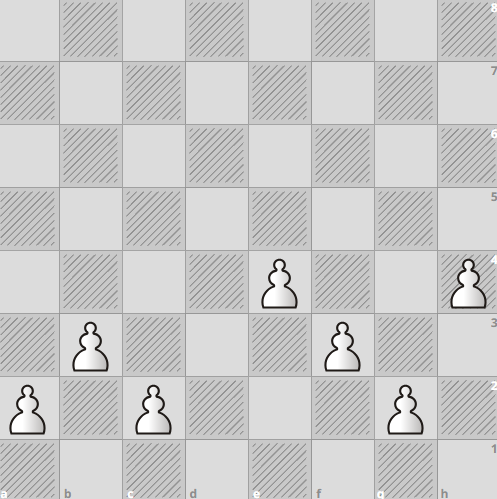
\includegraphics[scale=0.25]{images/PawnBitboard.png}
    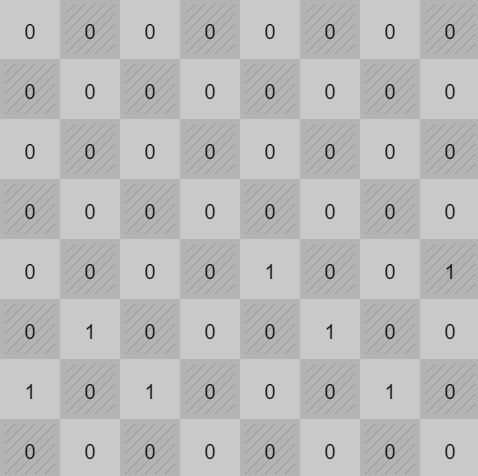
\includegraphics[scale=0.26]{images/PawnBitboardVals.png}
    \caption{Bitboard representation of the white pawns on the board}
    \label{fig: pawnBitboards}
\end{figure}

To represent a colour image, each pixel component (Red, Green, or Blue) is stored on a seperate "channel", this allows for dealing with each channel as a single layer in the case of grey-scale images, but instead of 0 being black and 255 being white, 255 would be the colour of the respective channel.

\begin{figure}[H]
    \centering
    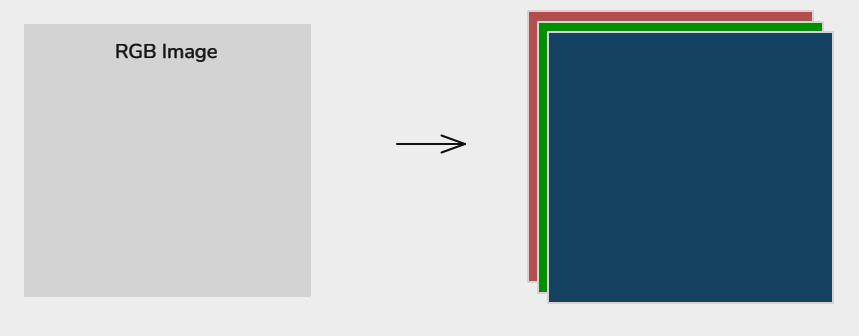
\includegraphics[scale=0.5]{images/RGBtoChannels.png}
    \caption{Decomposition of an RGB Image to Three Channels}
    \label{fig: RGBChannels}
\end{figure}

To represent an entire chess position one would need \textit{at least} 16 bitboards, one for each unique piece (white King, black King, white Queen, black Queen, and so on). Figure \ref{fig: Bitboards} shows a simplified version of this.

\begin{figure}[H]
    \centering
    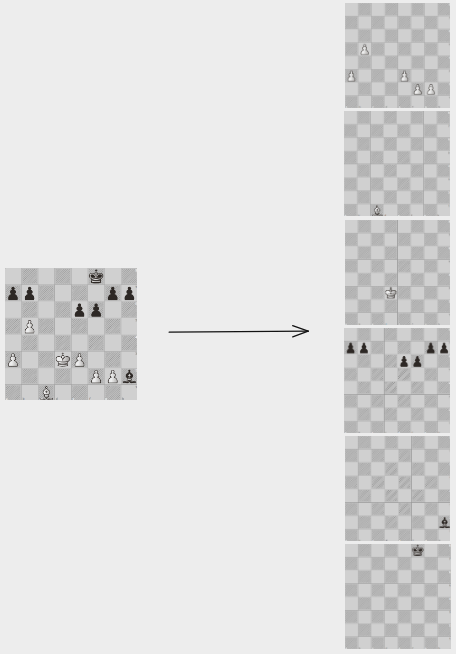
\includegraphics[scale=0.75]{images/BitboardDecomp.png}
    \caption{Decomposition of a position into various bitboards (here as actual pieces for simiplicity)}
    \label{fig: Bitboards}
\end{figure}
